\section*{The Database}

We investigate the plausibility of implementging $\cprobnext{X}$ as a search through a database of training data. We set up a database of known transitions between whisker shapes. A transition $T$ consists of a ``from'' state $f$ and a''to'' state $t$. This denotes that ``we have observed with 100\% accuracy that a whisker went from this shape to that shape in one time step''. We then approximate $\cprobnext{X}$ as a weighted average of the database, where transitions are weighted by how much their ``from'' parts differ from the hypotheses in $X_n$.

What we do in practice when sampling is: for each hypothesis $x_n^i \in X_n$,

\begin{enumerate}
  \item For each transition $T^j = (f^j, t^j)$ in the database, calculate the function $d^{ij}$ that is the difference between the two functions described by $x_n^i$ and $f^j$. In this case, both are polynomials and thus $d^{ij}$ is the polynomial with coefficients given by the tuple $x_n^i - f^i$.
  \item Let $w^{ij} = \left(\frac{1}{\norm{d^{ij}}_{\Ltwo}}\right)^a$, the reciprocal of the $\Ltwo$ norm of $d^{ij}$ raised to a power $a$.
  \item Return $\frac{\sum_j t^j w^{ij}}{\sum_jw^{ij}}$, the weighted average of the ``to'' states with weights $w^{ij}$.
\end{enumerate}

Doing this for each hypothesis $x_n^i$ yields the set $\bar{X}_n$.

\begin{figure}
  \centering
  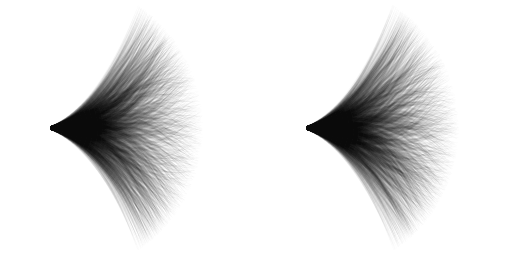
\includegraphics[width=0.7\textwidth]{database_gwhisker_spline3_n2048_from_to_fixed.png}
  \caption{View of all whiskers in transition database, from-states on the left and to-states on the right.}
  \label{fig:database}
\end{figure}
